\documentclass[tikz,border=6pt]{standalone}
\usepackage{amsmath}
\usepackage{xcolor}
\usetikzlibrary{arrows.meta,positioning}

\definecolor{axisgray}{HTML}{333333}
\definecolor{lineblue}{HTML}{4A90D9}
\definecolor{linered}{HTML}{E74C3C}
\definecolor{labelgreen}{HTML}{3C763D}

\begin{document}
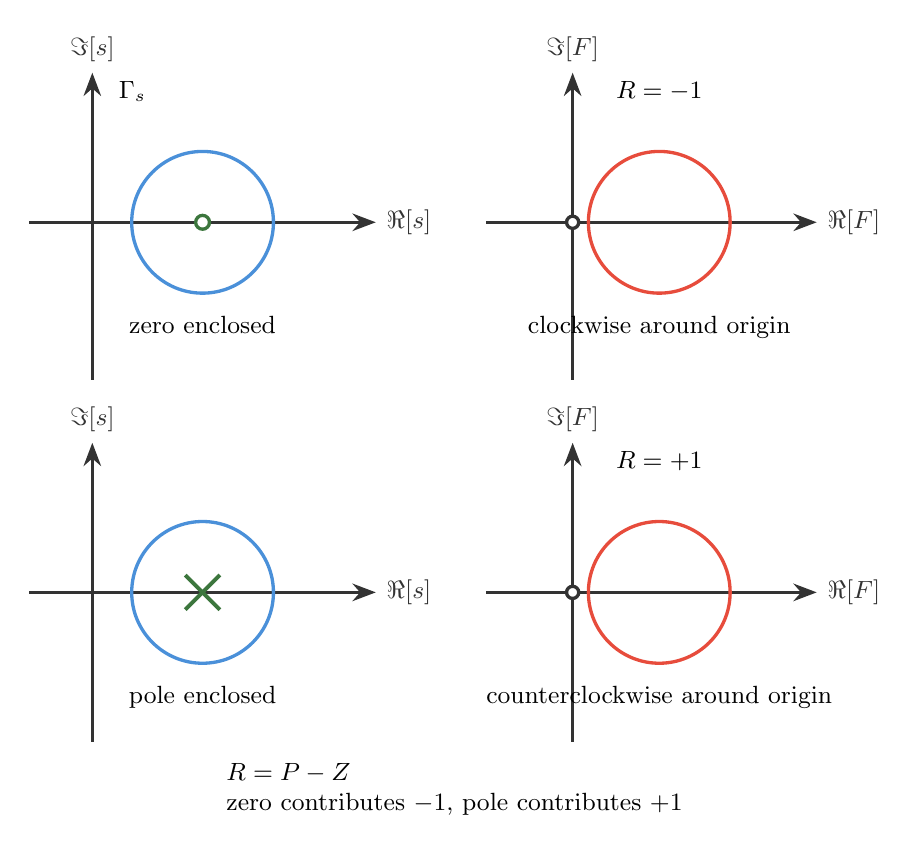
\begin{tikzpicture}[>=Stealth, line width=1.2pt, font=\small]
  \draw[axisgray, ->] (-0.8,1.6) -- (3.6,1.6) node[right] {$\Re[s]$};
  \draw[axisgray, ->] (0,-0.4) -- (0,3.5) node[above] {$\Im[s]$};
  \draw[lineblue, ->] (1.4,1.6) circle [radius=0.9];
  \filldraw[fill=white, draw=labelgreen] (1.4,1.6) circle (2.5pt);
  \node[below] at (1.4,0.55) {zero enclosed};
  \node[above right] at (0.2,3.0) {$\Gamma_s$};

  \draw[axisgray, ->] (5.0,1.6) -- (9.2,1.6) node[right] {$\Re[F]$};
  \draw[axisgray, ->] (6.1,-0.4) -- (6.1,3.5) node[above] {$\Im[F]$};
  \draw[linered, ->] (7.2,1.6) circle [radius=0.9];
  \filldraw[fill=white, draw=axisgray] (6.1,1.6) circle (2.2pt);
  \node[below] at (7.2,0.55) {clockwise around origin};
  \node[above] at (7.2,3.0) {$R=-1$};

  \draw[axisgray, ->] (-0.8,-3.1) -- (3.6,-3.1) node[right] {$\Re[s]$};
  \draw[axisgray, ->] (0,-5.0) -- (0,-1.2) node[above] {$\Im[s]$};
  \draw[lineblue, ->] (1.4,-3.1) circle [radius=0.9];
  \draw[labelgreen, line width=1.4pt] (1.18,-3.32) -- (1.62,-2.88);
  \draw[labelgreen, line width=1.4pt] (1.18,-2.88) -- (1.62,-3.32);
  \node[below] at (1.4,-4.15) {pole enclosed};

  \draw[axisgray, ->] (5.0,-3.1) -- (9.2,-3.1) node[right] {$\Re[F]$};
  \draw[axisgray, ->] (6.1,-5.0) -- (6.1,-1.2) node[above] {$\Im[F]$};
  \draw[linered, ->] (7.2,-3.1) circle [radius=0.9];
  \filldraw[fill=white, draw=axisgray] (6.1,-3.1) circle (2.2pt);
  \node[below] at (7.2,-4.15) {counterclockwise around origin};
  \node[above] at (7.2,-1.7) {$R=+1$};

  \node[align=left] at (4.6,-5.6) {$\displaystyle R=P-Z$\\zero contributes $-1$, pole contributes $+1$};
\end{tikzpicture}
\end{document}
